\documentclass{article}

\usepackage{graphicx}
\usepackage{fullpage}
\usepackage{wrapfig}
\usepackage{float}


\graphicspath{ {img/} }
\begin{document}

\title{Program 4 Design and Analysis}
\author{Julian Brackins, Ryan Feather, Joe Mowry and Charles Bonn}
\date{12/9/2014}
\maketitle

\section{Part 1 - Shared Memory}

\subsection{Program Description}

\subsection{Design}
Following Foster's design methodology, we have a brief overview:

\subsubsection{Partitioning}
        \begin{itemize}
            \item Reading values to be hashed
            \item Hashing
            \item Sending
            \item Recieving
            \item Inserting
        \end{itemize}
\subsubsection{Communication}
        \begin{itemize}
            \item Sharing data between computations
            \item Determine amount and pattern of communication
        \end{itemize}
\subsubsection{Aglomeration}
        \begin{itemize}
            \item Combine or group tasks to improve performance
        \end{itemize}
\subsubsection{Mapping}
        \begin{itemize}
            \item Assign agglomerated tasks to threads/physical processors.
        \end{itemize}


\subsection{Performance Testing}
The following figures overview the timing analysis for the shared memory solution for our hash table.
The raw data can be found in the timing analysis excel file in the documentation directory of
our project.
\begin{figure}[H]
  \caption{Timing Evaluation of increasing problem size}
  \centering
  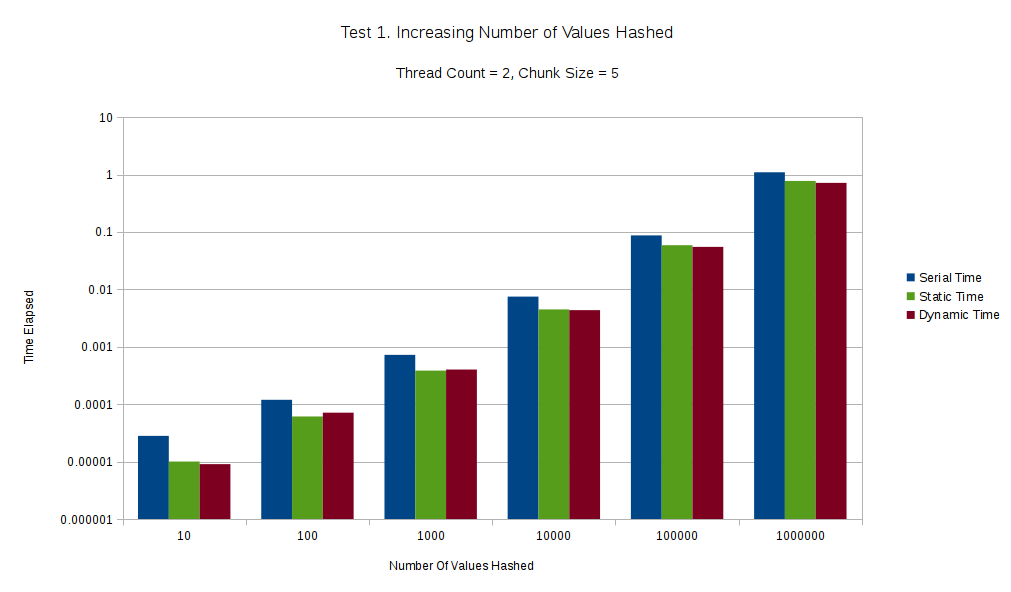
\includegraphics[width=\textwidth]{chart1a}
  \label{fig:chart1a}
\end{figure}

Figure~\ref{fig:chart1a} displays the timing evaluation of the shared memory hash table as the problem 
size is scaled up. In each run, the number of values added to the hash table are increased by a factor 
of 10. The strings added to the hash table are randomized, and every string is unique, since identical 
strings cannot be added to this hash table. As the problem size increases, the parallel solutions complete 
the tasks of inserting into the table faster than the serial solution.

\begin{figure}[H]
  \caption{Speedup / Efficiency Evaluation of increasing problem size}
  \centering
  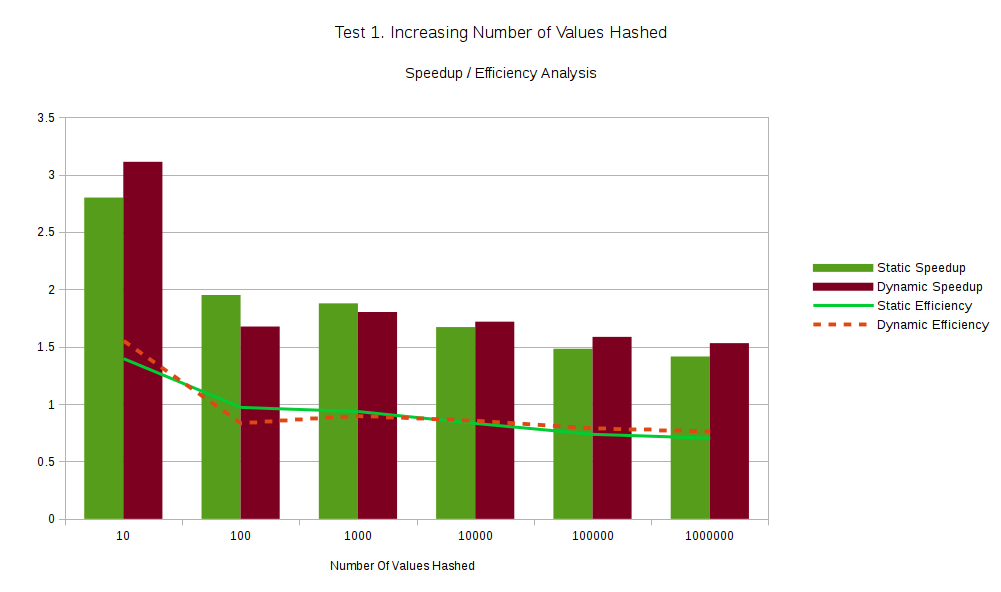
\includegraphics[width=\textwidth]{chart1b}
  \label{fig:chart1b}
\end{figure}

Figure~\ref{fig:chart1b} is the analysis of the speedup and efficiency gained by using the parallel solutions, 
both static and dynamic scheduling, on an increasing problem size. While we did observe in Figure~\ref{fig:chart1a} 
that the two parallel solutions were consistently faster than the serial counterpart, the actual speedup and 
efficiency observed as the problem size increases has a downward trend. Therefore, we can conclude that as the 
problem size increases, the speedup and efficiency of the parallel solution decreases, despite an overall better 
time performance.

\begin{figure}[H]
  \caption{Timing Evaluation of increasing thread count}
  \centering
  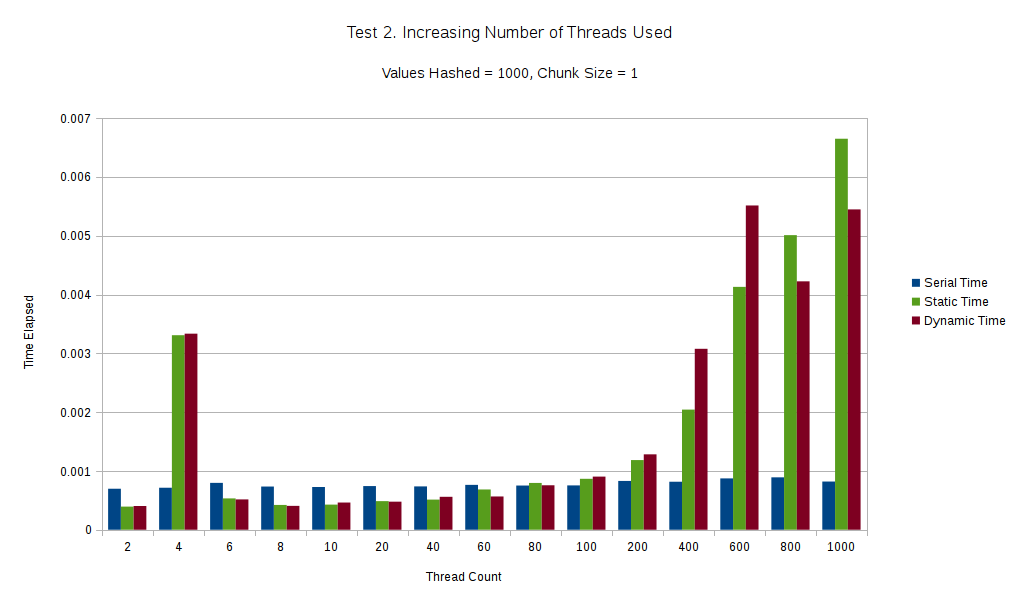
\includegraphics[width=\textwidth]{chart2a}
    \label{fig:chart2a}
\end{figure}

Figure~\ref{fig:chart2a} observes the timing evaluation of the shared memory hash table as the amount of threads 
increases. For smaller thread counts (2, 6 through around 60) the program overall has a better performance on the 
parallel versions as opposed to the serial method, but for larger thread counts (80+), the program actually 
performs better serially due to the amount of overhead from thread management. It should be noted that there is 
a rather peculiar spike in runtime for the parallel methods when running the program with 4 threads. For whatever 
reason, the program takes an incredibly long time when utilizing 4 threads, but returns to the expected trend 
with all other thread counts.

\begin{figure}[H]
  \caption{Speedup / Efficiency Evaluation of increasing thread count}
  \centering
  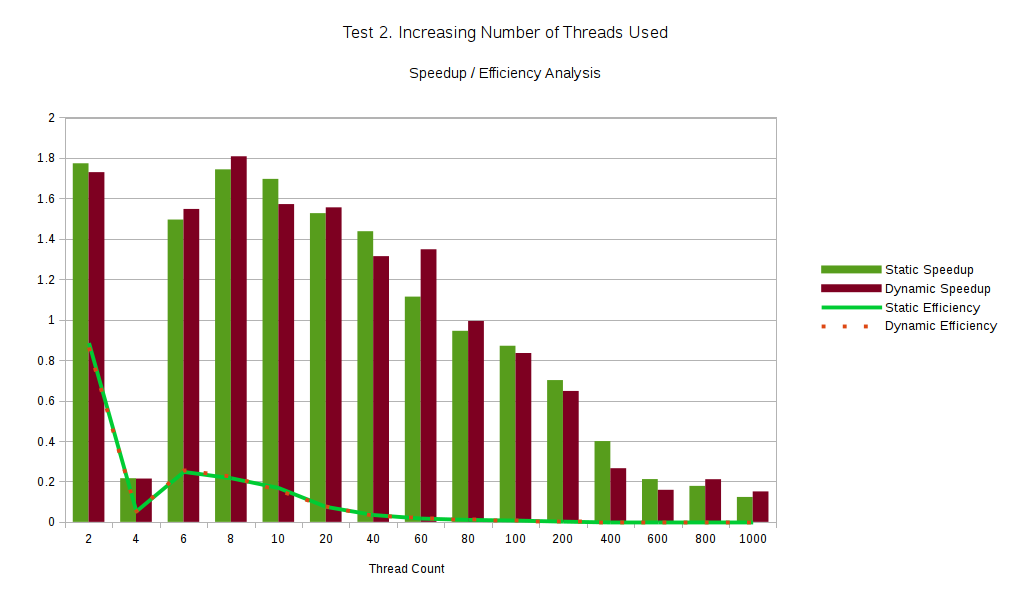
\includegraphics[width=\textwidth]{chart2b}
    \label{fig:chart2b}
\end{figure}

Figure~\ref{fig:chart2b} reflects this peculiar anomaly at a thread count of 4, but otherwise shows a mostly 
downward trend of both speedup and efficiency as more threads are used in the program. According to the chart, 
the Static scheduling method experiences the greatest speedup and efficiency at 2 threads. The Dynamic scheduling 
method, while technically having the greatest speedup rating at 8 threads, is most efficient at 2 threads as well.

\begin{figure}[H]
  \caption{Timing Evaluation of increasing chunk size}
  \centering
  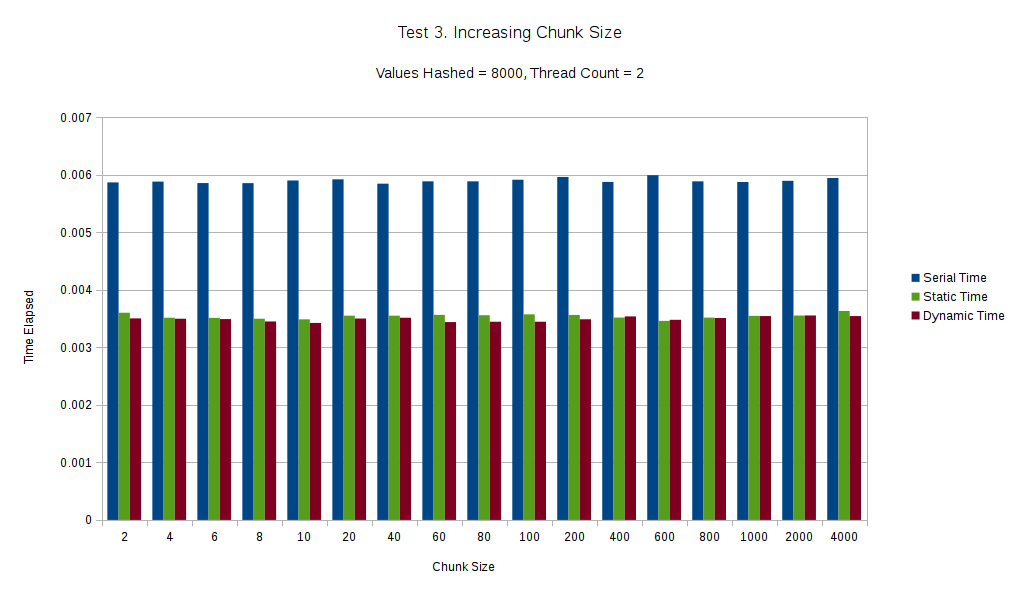
\includegraphics[width=\textwidth]{chart3a}
    \label{fig:chart3a}
\end{figure}

Figure~\ref{fig:chart3a} details the timings of the hash table inserts when the chunk size is increased on the 
parallel solutions. As this diagram illustrates, increasing chunk size has a somewhat noteworthy effect on the 
amount of time it takes for the program to run. Curiously, however, the amount of time required to run the program 
is basically identical over all tests as the chunk size increases. As long as the chunk size is greater than 1, the 
parallel solutions observe a faster runtime than the serial method, although this faster runtime is identical even 
as the chunk size increases.

\begin{figure}[H]
  \caption{Speedup / Efficiency Evaluation of increasing chunk size}
  \centering
  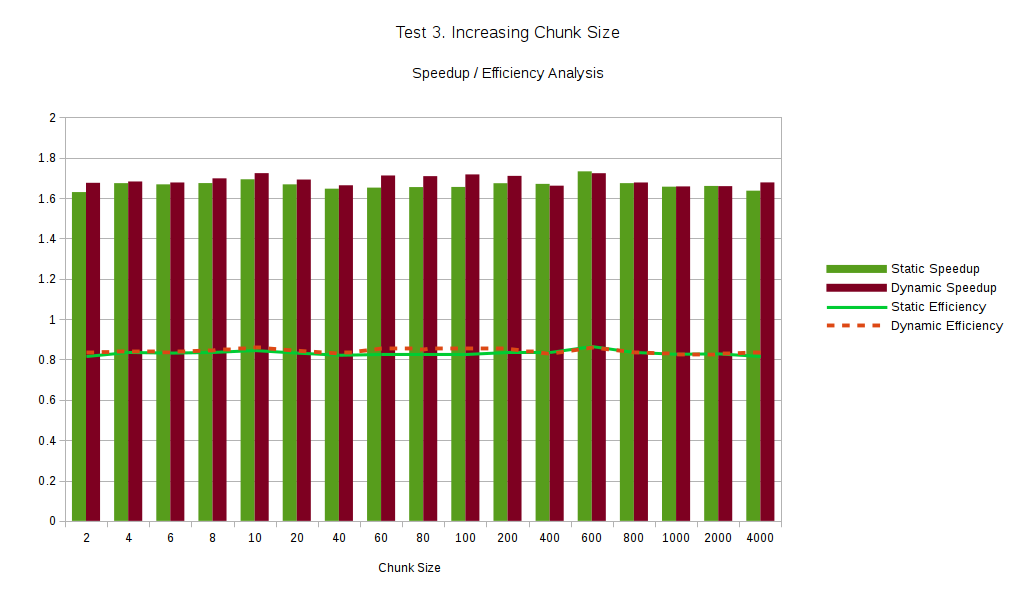
\includegraphics[width=\textwidth]{chart3b}
    \label{fig:chart3b}
\end{figure}

As a result of this observation, Figure~\ref{fig:chart3b} features a mostly horizontal trend in both speedup and efficiency as the chunk size given to each task increases in the parallel solution. 

\section{Part 2 - Distributed memory}
\subsection{Program Description}
This distributed memory program will allow for the typical hash table operations, but on a set of programs on potentially different computers.

Each process on each machine will be responsible for its own hash table, and respond to messages from a managing producer thread. The managing thread will give values to store and request table lookups.

The data is currently random strings read in from a file. A few sample inputs are provided.

\subsection{Design}
Following Foster's design methodology, we have a brief overview:

\subsubsection{Partitioning}
For our distributed memory solution, as in our shared, we will be doing data-centric partitioning. We will assign to each piece of data (in this case the strings) the tasks of hashing that data and storing it into a table. 

This will create a large number of tasks, much larger than our number of processors. There are no redundant computations, and each tak will be roughly the same size.

\subsubsection{Communication}
For each piece of data, in order to place it in a table, it must first be hashed according to the hash function. This is an example of local communication. Therfore, since the tasks are dependent, we can consolidate them into one single task, hashing and storing a value.

In addition, the tasks associated with a piece of data will work very independently. Very little global communication will be needed.

Communication is balanced, minimized, and all tasks can be performed concurrently.

\subsubsection{Aglomeration}
As discussed in the last section, each piece of data can be consolidated into one combined operation.

Other than that, there is not much agglomeration that can be done. Because the work associated with each piece of data is independint of the solution as a whole, and the locality of the table insert is minimal, we cannot group together tasks in a meaningful or advantageous way.

\subsubsection{Mapping}
For the distributed memory solution, we will employ a producer-consumer structure. We will have one root thread that produces values from an input file, handing out the values to the consumer threads. Each consumer thread will take the piece of data, hash it, and place it in the table.

It is very important that we balance the load that each consumer thread experiences, making sure that they are not overwhelemed with data that will make computation take longer or potentially fill up their table. At the same time, we want to make sure that the storing of data is determinstic, that way we can find the data in a later loopup operation. In order to do this, the data is hashed twice. Once by the root producer thread in order to determine which worker thread will get the data, and again by the worker to determine where in its table to place the data.



\subsection{Performance Testing}





\end{document}
